\documentclass[a4paper,12pt]{article}
\usepackage[indonesian]{babel}
\usepackage{graphicx}
\usepackage{multirow}
\usepackage{enumitem}
\usepackage{listings}
\usepackage{wrapfig}
\usepackage[T1]{fontenc}
\usepackage{inconsolata}
\usepackage{lipsum}
\usepackage{adjustbox}
\usepackage{upquote}


\usepackage{color}
\usepackage[table]{xcolor}
\definecolor{lightgray}{rgb}{0.95, 0.95, 0.95}
\definecolor{darkgray}{rgb}{0.4, 0.4, 0.4}
%\definecolor{purple}{rgb}{0.65, 0.12, 0.82}
\definecolor{editorGray}{rgb}{0.95, 0.95, 0.95}
\definecolor{editorOcher}{rgb}{1, 0.5, 0} % #FF7F00 -> rgb(239, 169, 0)
\definecolor{editorGreen}{rgb}{0, 0.5, 0} % #007C00 -> rgb(0, 124, 0)
\definecolor{orange}{rgb}{1,0.45,0.13}		
\definecolor{olive}{rgb}{0.17,0.59,0.20}
\definecolor{brown}{rgb}{0.69,0.31,0.31}
\definecolor{purple}{rgb}{0.38,0.18,0.81}
\definecolor{lightblue}{rgb}{0.1,0.57,0.7}
\definecolor{lightred}{rgb}{1,0.4,0.5}
% CSS
\lstdefinelanguage{CSS}{
  keywords={color,background-image:,margin,padding,font,weight,display,position,top,left,right,bottom,list,style,border,size,white,space,min,width, transition:, transform:, transition-property, transition-duration, transition-timing-function},	
  sensitive=true,
  morecomment=[l]{//},
  morecomment=[s]{/*}{*/},
  morestring=[b]',
  morestring=[b]",
  alsoletter={:},
  alsodigit={-}
}

% JavaScript
\lstdefinelanguage{JavaScript}{
  morekeywords={typeof, new, true, false, catch, function, return, null, catch, switch, var, if, in, while, do, else, case, break},
  morecomment=[s]{/*}{*/},
  morecomment=[l]//,
  morestring=[b]",
  morestring=[b]'
}

\lstdefinelanguage{HTML5}{
  language=html,
  sensitive=true,	
  alsoletter={<>=-},	
  morecomment=[s]{<!-}{-->},
  tag=[s],
  otherkeywords={
  % General
  >,
  % Standard tags
	<!DOCTYPE,
  </html, <html, <head, <title, </title, <style, </style, <link, </head, <meta, />,
	% body
	</body, <body,
	% Divs
	</div, <div, </div>, 
	% Paragraphs
	</p, <p, </p>,
	% scripts
	</script, <script,
  % More tags...
  <canvas, /canvas>, <svg, <rect, <animateTransform, </rect>, </svg>, <video, <source, <iframe, </iframe>, </video>, <image, </image>, <header, </header, <article, </article
  },
  ndkeywords={
  % General
  =,
  % HTML attributes
  charset=, src=, id=, width=, height=, style=, type=, rel=, href=,
  % SVG attributes
  fill=, attributeName=, begin=, dur=, from=, to=, poster=, controls=, x=, y=, repeatCount=, xlink:href=,
  % properties
  margin:, padding:, background-image:, border:, top:, left:, position:, width:, height:, margin-top:, margin-bottom:, font-size:, line-height:,
	% CSS3 properties
  transform:, -moz-transform:, -webkit-transform:,
  animation:, -webkit-animation:,
  transition:,  transition-duration:, transition-property:, transition-timing-function:,
  }
}

\lstdefinestyle{htmlcssjs} {%
  % General design
%  backgroundcolor=\color{editorGray},
  basicstyle={\footnotesize\ttfamily},   
  frame=single,
  % line-numbers
  % Code design
  identifierstyle=\color{black},
  keywordstyle=\color{blue}\bfseries,
  ndkeywordstyle=\color{editorGreen}\bfseries,
  stringstyle=\color{editorOcher}\ttfamily,
  commentstyle=\color{brown}\ttfamily,
  % Code
  language=HTML5,
  alsolanguage=JavaScript,
  alsodigit={.:;},	
  tabsize=2,
  showtabs=false,
  showspaces=false,
  showstringspaces=false,
  extendedchars=true,
  breaklines=true,
  % German umlauts
  literate=%
  {Ö}{{\"O}}1
  {Ä}{{\"A}}1
  {Ü}{{\"U}}1
  {ß}{{\ss}}1
  {ü}{{\"u}}1
  {ä}{{\"a}}1
  {ö}{{\"o}}1
}
%
\lstdefinestyle{py} {%
language=python,
literate=%
*{0}{{{\color{lightred}0}}}1
{1}{{{\color{lightred}1}}}1
{2}{{{\color{lightred}2}}}1
{3}{{{\color{lightred}3}}}1
{4}{{{\color{lightred}4}}}1
{5}{{{\color{lightred}5}}}1
{6}{{{\color{lightred}6}}}1
{7}{{{\color{lightred}7}}}1
{8}{{{\color{lightred}8}}}1
{9}{{{\color{lightred}9}}}1,
basicstyle=\footnotesize\ttfamily, % Standardschrift
numbers=left,               % Ort der Zeilennummern
%numberstyle=\tiny,          % Stil der Zeilennummern
%stepnumber=2,               % Abstand zwischen den Zeilennummern
numbersep=5pt,              % Abstand der Nummern zum Text
tabsize=4,                  % Groesse von Tabs
extendedchars=true,         %
breaklines=true,            % Zeilen werden Umgebrochen
keywordstyle=\color{blue}\bfseries,
frame=b,
commentstyle=\color{brown}\itshape,
stringstyle=\color{editorOcher}\ttfamily, % Farbe der String
showspaces=false,           % Leerzeichen anzeigen ?
showtabs=false,             % Tabs anzeigen ?
xleftmargin=17pt,
framexleftmargin=17pt,
framexrightmargin=5pt,
framexbottommargin=4pt,
%backgroundcolor=\color{lightgray},
showstringspaces=false,      % Leerzeichen in Strings anzeigen ?
}%
%
\definecolor{dkgreen}{rgb}{0,.6,0}
\definecolor{dkblue}{rgb}{0,0,.6}
\definecolor{dkyellow}{cmyk}{0,0,.8,.3}

\lstdefinestyle{PHP}{
  language        = php,
  basicstyle      = \small\ttfamily,
  keywordstyle    = \color{dkblue},
  stringstyle     = \color{red},
  identifierstyle = \color{dkgreen},
  commentstyle    = \color{gray},
  emph            =[1]{php},
  emphstyle       =[1]\color{black},
  emph            =[2]{if,and,or,else},
  emphstyle       =[2]\color{dkyellow}}
\lstset{
    showstringspaces=false,
    frame=single,
    breaklines=true,
    rulecolor=\color{black},
    style=htmlcssjs
}
%

\graphicspath{ {./img/} }
\begin{document}
\title{ {\Large Tugas 12}\\ Pemrograman Web Client\\{\Large Pertemuan 12}}

\author{Aldzikri Dwijayanto Prathama 
	\\195410189
	\\Informatika}
\makeatletter
\begin{titlepage}
	\begin{center}
		{\huge \bfseries \@title }\\[14ex]
		
\includegraphics[scale=.8]{logo}\\[4ex]
		{\large \@author}\\[12ex]
		{\large \bfseries {SEKOLAH TINGGI MANAJEMEN INFORMATIKA DAN KOMPUTER
				AKAKOM YOGYAKARTA}}
	\end{center}


%{\large \@date} 
\end{titlepage}
\makeatother
%\maketitle
\renewcommand{\figurename}{Gambar}
\newpage

\section*{DOM Methods}
DOM Method adalah tindakan yang dapat dilakukan pada Elemen HTML.\@ Properti DOMnya yaitu nilai dari Element yang dapat
kita atur atau ubah. DOM dapat diakses dengan JavaScript dan dengan bahasa pemrograman lain. Pada DOM, semua elemen HTML
didefinisikan sebagai objek.

\begin{lstlisting}[style=htmlcssjs]
<!DOCTYPE html>
<html>
    <body>
        <h2>My First Page</h2>
        <p id="demo"></p>

   <script>
       document.getElementById("demo").innerHTML = "Hello World!";
   </script>

    </body>
</html>
\end{lstlisting}
\begin{center}
    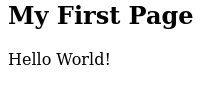
\includegraphics[scale=.7]{1.png} 
\end{center}

\section*{DOM Document}
DOM Document object adalah inti dari objek lain di halaman web yang kita buat. Objek dokumen menggambarkan bagaimana
halaman web yang dibuat. Jika kita ingin mengakses elemen apa pun di halaman HTML, langkah awal yang dilakukan adalah
dengan mengakses objek dokumen.

\section*{DOM Elements}
Seringkali, dengan JavaScript, kita ingin memanipulasi elemen HTML.\@ Untuk melakukannya, kita harus menemukan elemen
elemennya terlebih dahulu. Ada beberapa cara untuk melakukan ini, yaitu dengan: Menemukan elemen HTML melalui id
\begin{itemize}
 \item Menemukan elemen HTML dengan nama tag
 \item Menemukan elemen HTML dengan nama class
 \item Menemukan elemen HTML oleh CSS selektor
 \item Menemukan elemen HTML dengan HTML object collections
\end{itemize}
\begin{lstlisting}
<!DOCTYPE html>
<html>
    <body>
        <h2>Finding HTML Elements by Id</h2>

        <p id="intro">Hello World!</p>
        <p>This example demonstrate the <b>getElementById</b> method.</p>
        <p id="demo"></p>

   <script>
       var myElement = document.getElementById("intro");
       document.getElementById("demo").innerHTML = 
           "The text from the intro paragraph is " + myElement.innerHTML;
   </script>

    </body>
</html>
\end{lstlisting}

\begin{center}
    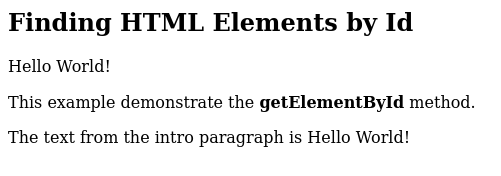
\includegraphics[scale=.7]{2.png} 
\end{center}

\section*{DOM HTML}
DOM HTML memungkinkan JavaScript untuk mengubah konten elemen HTML. JavaScript dapat membuat konten HTML dinamis seperti
contoh berikut, yang akan menampilkan waktu laman dimuat.
\begin{lstlisting}
<!DOCTYPE html>
<html>
    <body>
   <script>
       document.write(Date());
   </script>
    </body>
</html>

\end{lstlisting}

\begin{center}
    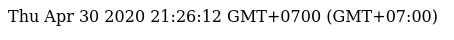
\includegraphics[scale=.7]{3.png} 
\end{center}

\section*{DOM CSS}
DOM CSS memungkinkan JavaScript untuk mengubah gaya elemen HTML.
Contoh berikut mengubah gaya elemen <p>:
\begin{lstlisting}
<!DOCTYPE html>
<html>
    <body>
        <p id="p1">Hello World!</p>
        <p id="p2">Hello World!</p>

    <script>
        document.getElementById("p2").style.color="blue";
        document.getElementById("p2").style.fontFamily="Arial";
        document.getElementById("p2").style.fontSize="larger";
    </script>

    <p>The paragraph above was changed by a script</p>
    </body>

</html>

</html>
\end{lstlisting}

\begin{center}
    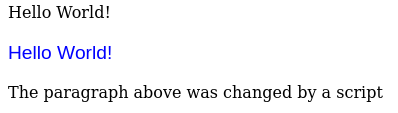
\includegraphics[scale=.7]{4.png} 
\end{center}

\section*{DOM Animation}
DOM Animation dilakukan dengan memprogram perubahan bertahap dalam element style. Perubahan itu disebut dengan timer. Ketika interval timer kecil, animasi terlihat terus menerus.
\begin{lstlisting}
<!DOCTYPE html>
<html>
<style>
#container {
  width: 400px;
  height: 400px;
  position: relative;
  background: yellow;
}
#animate {
  width: 50px;
  height: 50px;
  position: absolute;
  background-color: red;
}
</style>
<body>

<p><button onclick="myMove()">Click Me</button></p> 

<div id ="container">
  <div id ="animate"></div>
</div>

<script>
function myMove() {
  var elem = document.getElementById("animate");   
  var pos = 0;
  var id = setInterval(frame, 5);
  function frame() {
    if (pos == 350) {
      clearInterval(id);
    } else {
      pos++; 
      elem.style.top = pos + "px"; 
      elem.style.left = pos + "px"; 
    }
  }
}
</script>

</body>
</html>
\end{lstlisting}
\begin{center}
    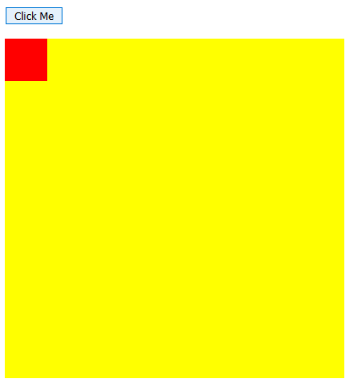
\includegraphics[scale=.7]{anim1.png} 
    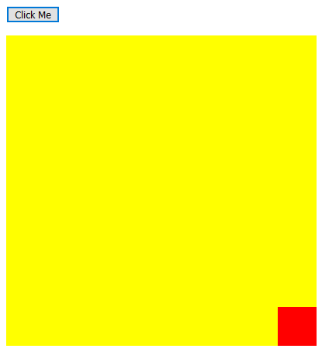
\includegraphics[scale=.7]{anim2.png} 
\end{center}

\section*{DOM Events}
JavaScript dapat dieksekusi ketika suatu peristiwa terjadi, seperti ketika pengguna mengklik elemen HTML.\@
Contoh HTML Event:
\begin{itemize}
 \item Ketika pengguna mengklik mouse
 \item Ketika halaman web telah dimuat
 \item Ketika suatu gambar telah dimuat
 \item Saat mouse bergerak di atas elemen
 \item Ketika bidang input diubah
 \item Ketika formulir HTML dikirimkan
 \item Saat pengguna menekan tombol
\end{itemize}
Dalam contoh ini, konten elemen <h1> berubah ketika pengguna mengkliknya:
\begin{lstlisting}
<!DOCTYPE html>
<html>
    <body>
        <h1 onclick="this.innerHTML='Ooops!'">Click on this text!</h1>
    </body>
</html>
\end{lstlisting}

\begin{center}
    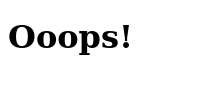
\includegraphics[scale=.7]{5.png} 
\end{center}

\section*{DOM Event Listener}
addEventListener() method melampirkan event handler ke elemen yang ditentukan dan tanpa menimpa event handler yang ada. Kita dapat menambahkan banyak event handles ke satu elemen. Kita juga dapat menambahkan banyak event handles dari jenis yang sama ke satu elemen, yaitu dua "klik" events. Kemudian kita dapat menambahkan event listener ke objek DOM apa pun, tidak hanya elemen HTML. Yaitu object.
\begin{lstlisting}
<!DOCTYPE html>
<html>
    <body>
        <h2>Javascript addEventListener()</h2>
        <p>This example uses the addEventListener() method to attach a click event to a button.</p>
        <button id="myBtn">Try it</button>
        <p id="demo"></p>
        <script>
            document.getElementById("myBtn").addEventListener("click",displayDate);

            function displayDate() {
                document.getElementById("demo").innerHTML=Date();
            }
        </script>
    </body>
</html>
\end{lstlisting}

\begin{center}
    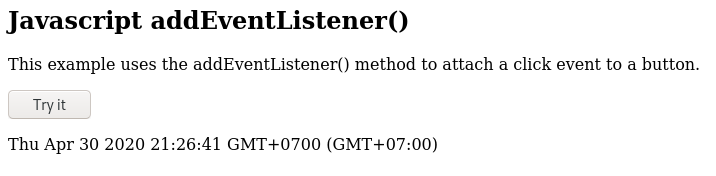
\includegraphics[scale=.7]{6.png} 
\end{center}

\section*{DOM Navigation}
Dengan HTML DOM, kita dapat menavigasi node pohon menggunakan hubungan node. Menurut standar HTML DOM W3C, segala sesuatu dalam dokumen HTML adalah sebuah node:
\begin{itemize}
    \item Seluruh dokumen adalah simpul dokumen
    \item Setiap elemen HTML adalah simpul elemen
    \item Teks di dalam elemen HTML adalah node teks
    \item Setiap atribut HTML adalah simpul atribut (tidak digunakan lagi)
    \item Semua komentar adalah simpul komentar
\end{itemize}
Dengan HTML DOM, semua node di dalam pohon node dapat diakses oleh JavaScript. Node baru dapat dibuat, dan semua node dapat dimodifikasi atau dihapus. Node dalam pohon node memiliki hubungan hirarkis satu sama lain. Istilah orang tua, anak, dan saudara kandung digunakan untuk menggambarkan hubungan.
\begin{lstlisting}
<!DOCTYPE html>
<html>
    <body>
        <h1 id="id01">My First Page</h1>
        <p id="id02"></p>

        <script>
            document.getElementById("id02").innerHTML = document.getElementById("id02").innerHTML;
        </script>
    </body>
</html>
\end{lstlisting}

\begin{center}
    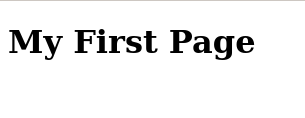
\includegraphics[scale=.7]{7.png} 
\end{center}

\section*{DOM Nodes}
Untuk menambahkan elemen baru ke HTML DOM, Anda harus membuat elemen (elemen node) terlebih dahulu, lalu menambahkannya ke elemen yang sudah ada.
\begin{lstlisting}
<!DOCTYPE html>
<html>
    <body>
        <div id="div1">
            <p id="p1">This is a paragraph</p>
            <p id="p2">This is another paragraph</p>
        </div>
   <script>
       var para = document.createElement("p");
       var node = document.createTextNode("this id new.");
       para.appendChild(node);
       var element = document.getElementById("div1");
       element.appendChild(para);
   </script>
    </body>
</html>
\end{lstlisting}
\begin{center}
    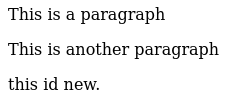
\includegraphics[scale=.7]{8.png} 
\end{center}

\section*{DOM Collection}
Metode getElementsByTagName() mengembalikan objek HTMLCollection. Objek HTMLCollection adalah daftar (koleksi) elemen mirip-array dari HTML 
HTML DOM Collection mungkin terlihat seperti array, tetapi tidak kita dapat mengulang daftar dan merujuk elemen dengan angka (seperti array). Namun, kita tidak dapat menggunakan metode array seperti valueOf(), pop(), push(), atau join() pada HTML Collection.
\begin{lstlisting}
<!DOCTYPE html>
<html>
<body>

<h2>JavaScript HTML DOM</h2>

<p>Hello World!</p>

<p>Hello Norway!</p>

<p>Click the button to change the color of all p elements.</p>

<button onclick="myFunction()">Try it</button>

<script>
function myFunction() {
  var myCollection = document.getElementsByTagName("p");
  var i;
  for (i = 0; i < myCollection.length; i++) {
    myCollection[i].style.color = "red";
  }
}
</script>

</body>
</html>
\end{lstlisting}
\begin{center}
    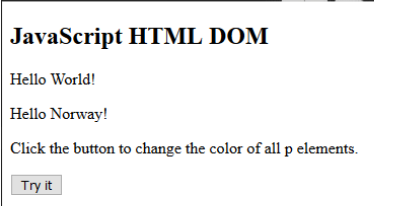
\includegraphics[scale=.7]{col1.png} 
    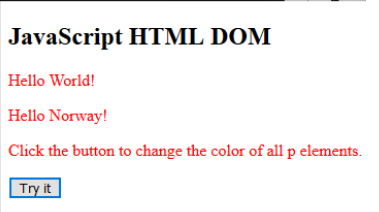
\includegraphics[scale=.7]{col2.png} 
\end{center}

\section*{DOM Node List}
Objek NodeList adalah daftar (kumpulan) node yang diekstrak dari dokumen. Objek NodeList hampir sama dengan objek HTMLCollection. Beberapa browser (yang lebih lama) mengembalikan objek NodeList alih-alih HTMLCollection untuk metode seperti getElementsByClassName(). Semua browser mengembalikan objek NodeList untuk childNodes properti. Sebagian besar browser mengembalikan objek NodeList untuk metode querySelectorAll (). HTML DOM Node list juga bukan array.
\begin{lstlisting}
<!DOCTYPE html>
<html>
<body>

<h2>JavaScript HTML DOM!</h2>

<p>Hellow World!</p>

<p>Hellow Norway!</p>

<p id="demo"></p>

<script>
var myNodelist = document.querySelectorAll("p");
document.getElementById("demo").innerHTML =
"This document contains " + myNodelist.length + " paragraphs.";
</script>

</body>
</html>
\end{lstlisting}
\begin{center}
    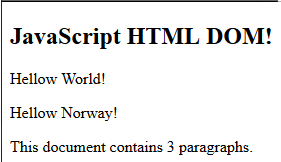
\includegraphics[scale=.7]{node.png} 
\end{center}

\end{document}
